%\documentclass[handout, xcolor={table, dvipsnames}]{beamer}
\documentclass[9pt, xcolor={table, dvipsnames}]{beamer}

\usepackage{fix-cm} % HUGE font size:\fontsize{50}{60}\selectfont
\usetheme{Warsaw}
%\usetheme{Frankfurt}
%\usetheme{Rochester}
%\usecolortheme{seagull}
%\usecolortheme[RGB={205,173,0}]{structure} 

%\usepackage{mathtools} %%% Conflict with xparse !!!!!!
\usepackage{marvosym}
\usepackage[utf8]{inputenc}
\usepackage{graphicx}
\usepackage{listings}
\usepackage{tikz}
\usetikzlibrary{bayesnet} 
\usepackage{bm}
\usepackage{bbm}
\usepackage{multirow}
\usepackage{booktabs}
\usepackage{subfigure}


%%%%%%%%%%% Box 
\usepackage{calc}%    For the \widthof macro
\usepackage{xparse}%  For \NewDocumentCommand
\newcommand{\tikzmark}[1]{\tikz[overlay,remember picture] \node (#1) {};}
\usecolortheme[named=OliveGreen]{structure} 
\setbeamertemplate{items}[ball] 
\setbeamertemplate{blocks}[rounded][shadow=true] 
%\setbeamertemplate{headline}{} % no ToC on top of each slides
\setbeamertemplate{navigation symbols}{} % To remove the navigation symbols from the bottom of all slides uncomment this line 
\addtobeamertemplate{footline}{\hfill~~\insertframenumber/\inserttotalframenumber~~}
%\setbeamertemplate{footline}[page number] % To replace the footer line in all slides with a simple slide count uncomment this line 

%\useoutertheme{infolines} 
\setbeamercolor{mini frame}{fg=darkred} % marche pas!!!

\makeatletter
\def\insertsubsectionnavigationhorizontal#1#2#3{%
    \hbox to #1{{%
        \usebeamerfont{subsection in head/foot}\usebeamercolor[fg]{subsection in head/foot}
        \beamer@currentsubsection=0%
        \def\sectionentry##1##2##3##4##5{}%
        \def\slideentry##1##2##3##4##5##6{\ifnum##6=\c@part\ifnum##1=\c@section%
      \ifnum##2>\beamer@currentsubsection%
      \box\beamer@sectionbox\hskip1.875ex plus1fill%
            \hbox to 0pt{%
                    \global\beamer@section@min@dim\beamer@tempdim
                        \beamer@link(##4){%
                            \usebeamerfont{mini frame}%
                            \ifnum\c@section=##1%
                                \ifnum\c@subsection=##2%
                                    \usebeamercolor[fg]{mini frame}%
                                    \ifnum\c@subsectionslide=##3%
                                        \usebeamertemplate{mini frame}%\beamer@minislidehilight%
                                    \else%
                                        \usebeamertemplate{mini frame in current subsection}%\beamer@minisliderowhilight%
                                    \fi%
                                \else%
                                    \usebeamercolor{mini frame}%
                                    %\color{fg!50!bg}%
                                    \usebeamertemplate{mini frame in other subsection}%\beamer@minislide%
                                \fi%
                            \else%
                                \usebeamercolor{mini frame}%
                                                                %\color{fg!50!bg}%
                                \usebeamertemplate{mini frame in other subsection}%\beamer@minislide%
                            \fi%
                        }%
                \hskip-10cm plus 1fil%
            }%
            \fi\fi\fi\ignorespaces
        }%
        #2\hskip.3cm\setbox\beamer@sectionbox=\hbox{}%
        \hskip-1.875ex plus-1fill\dohead%
        \box\beamer@sectionbox\hfil\hskip.3cm%
        #3
    }}
}
\makeatother

\setbeamertemplate{headline}
{
  \leavevmode%
  \hbox{%
  \begin{beamercolorbox}[wd=.5\paperwidth,ht=2.65ex,dp=1.5ex,right]{section in head/foot}%
    \usebeamerfont{section in head/foot}\bfseries\insertsectionhead\hspace*{2ex}
  \end{beamercolorbox}%
  \begin{beamercolorbox}[wd=.5\paperwidth,ht=2.65ex,dp=1.5ex,left]{subsection in head/foot}%
    \usebeamerfont{subsection in head/foot}\setbeamercolor{section in head/foot}{fg=black,bg=white}
    \vspace*{.01cm}\insertsubsectionnavigationhorizontal{1cm}{\hskip-.1cm}{}
  \end{beamercolorbox}}%
  \vskip0pt%
}

\setbeamertemplate{footline}
{
    \leavevmode%
    \hbox{%
        \begin{beamercolorbox}[wd=.333333\paperwidth,ht=2.25ex,dp=1ex,right]{author in head/foot}%
            \usebeamerfont{author in head/foot}\insertshortauthor\hspace{2ex}~~%\beamer@ifempty{\insertshortinstitute}{}{(\insertshortinstitute)}
        \end{beamercolorbox}%
        \begin{beamercolorbox}[wd=.588888\paperwidth,ht=2.25ex,dp=1ex,left]{title in head/foot}%
            \hspace{2ex}\usebeamerfont{title in head/foot}\insertshorttitle
        \end{beamercolorbox}%
        \begin{beamercolorbox}[wd=.088888\paperwidth,ht=2.25ex,dp=1ex,right]{date in head/foot}%
            \insertframenumber{} / \inserttotalframenumber\hspace*{2ex}~~
    \end{beamercolorbox}}%
    \vskip0pt%
}

%\usepackage[footheight=1em]{beamerthemeboxes}
%\addfootboxtemplate{\color{black}}{\color{white}\hfill\insertframenumber/\inserttotalframenumber\hspace{2em}\null}

\AtBeginSection[]
{
  \begin{frame}<beamer>
    \frametitle{Summary}
    \tableofcontents[currentsection, currentsubsection]
  \end{frame}
}

\AtBeginSubsection[]
{
  \begin{frame}<beamer>
    \frametitle{Sommaire}
    \tableofcontents[currentsection, currentsubsection]
  \end{frame}
}

% Variable de compilation
\newif\ifbeamer
\beamertrue
\newcommand{\beamer}[2]{\ifbeamer #1 \else #2 \fi}
%%%

   

\makeatletter
\NewDocumentCommand{\DrawBox}{s O{}}{%
    \tikz[overlay,remember picture]{
    \IfBooleanTF{#1}{%
        \coordinate (RightPoint) at ($(left |- right)+(\linewidth-\labelsep-\labelwidth,0.0)$);
    }{%
        \coordinate (RightPoint) at (right.east);
    }%
    \draw[red,#2]
      ($(left)+(-0.2em,0.9em)$) rectangle
      ($(RightPoint)+(0.2em,-0.3em)$);}
}

\NewDocumentCommand{\DrawBoxWide}{s O{}}{%
    \tikz[overlay,remember picture]{
    \IfBooleanTF{#1}{%
        \coordinate (RightPoint) at ($(left |- right)+(\linewidth-\labelsep-\labelwidth,0.0)$);
    }{%
        \coordinate (RightPoint) at (right.east);
    }%
    \draw[red,#2]
      ($(left)+(-\labelwidth,0.9em)$) rectangle
      ($(RightPoint)+(0.2em,-0.3em)$);}
}
\makeatother
%%%%% ! Box


\lstnewenvironment{C}[1]
{\lstset{language=C,
      frame=tBRl,
      basicstyle=\ttfamily\scriptsize,stringstyle=\emph,showstringspaces=false,
      numbers=left,numberstyle=\tiny,
      breaklines=true, columns=flexible, title={#1}}
}{}
\lstnewenvironment{C1}[1]
{\lstset{language=C,
      frame=tBRl,
      basicstyle=\ttfamily\scriptsize,stringstyle=\emph,showstringspaces=false,
      breaklines=true, columns=flexible, title={#1}}
}{}

\lstset{language=C,
  basicstyle=\ttfamily\tiny,%scriptsize,
  columns=flexible}

\newtheorem{Problemes}{Problèmes}
\newtheorem{Avantages}{Avantages}
\newtheorem{Inconvenients}{Inconvénients}

\title{A study of stochastic mixed membership models for link prediction in social networks}
\subtitle{---\\}
\author[Dulac Adrien]{Dulac Adrien\\[3mm] Christine Largeron -- Eric Gaussier}
\date{Octobre 2017}
\institute{LIG / AMA}

\usepackage[backend=bibtex]{biblatex}
\addbibresource{a.bib}

\begin{document}

\begin{frame}
    \titlepage
    \begin{tikzpicture}[overlay, remember picture]
\node[anchor=south west, %anchor is upper left corner of the graphic
      xshift=1em, 
      yshift=20pt] 
     at (current page.south west) %left upper corner of the page
    {
        
\includegraphics[scale=0.20]{./img/logo-arc6.png}
    };
\end{tikzpicture}
\begin{tikzpicture}[overlay, remember picture]
\node[anchor=south, %anchor is upper left corner of the graphic
      xshift=0em, 
      yshift=20pt] 
     at (current page.south) %left upper corner of the page
    {
        
\includegraphics[scale=0.20]{./img/logo-uga.png}
    };
\end{tikzpicture}
\begin{tikzpicture}[overlay, remember picture]
\node[anchor=south east, %anchor is upper left corner of the graphic
      xshift=-5em, 
      yshift=20pt] 
     at (current page.south east) %left upper corner of the page
    {
        
\includegraphics[scale=0.18]{./img/logo-alps.png}
    };
\end{tikzpicture}
 
\end{frame}

%\begin{frame}
%are ML and statistics complementary
%\end{frame}

%@Debug
%   * add properties and  formalism in 2. Gives interpretation analytic?local (convex survival) geometric?global (rich get richer)
%   * slide burstiness citation ?
%   * speech, bustiness vs sparsity ?

\begin{frame}{Table of contents}
    \tableofcontents
\end{frame}


%%%%%%%%%%%%%%%%%%%%%%%%%%%%%%%%%%%%%%%%%%%%
\section{Introduction}
%%%%%%%%%%%%%%%%%%%%%%%%%%%%%%%%%%%%%%%%%%%%

%
% * Networks are a type of structure data.
% * They represent relationnal data (dyadyc, interconected data ?)
% * arise in a lot of domains :
%   * sciologi, business, biology, etc... 
% complex because structure not wel defined as planar graph, trees etc
%

\begin{frame}[c]{Complex Networks}
    \begin{figure}[h]
    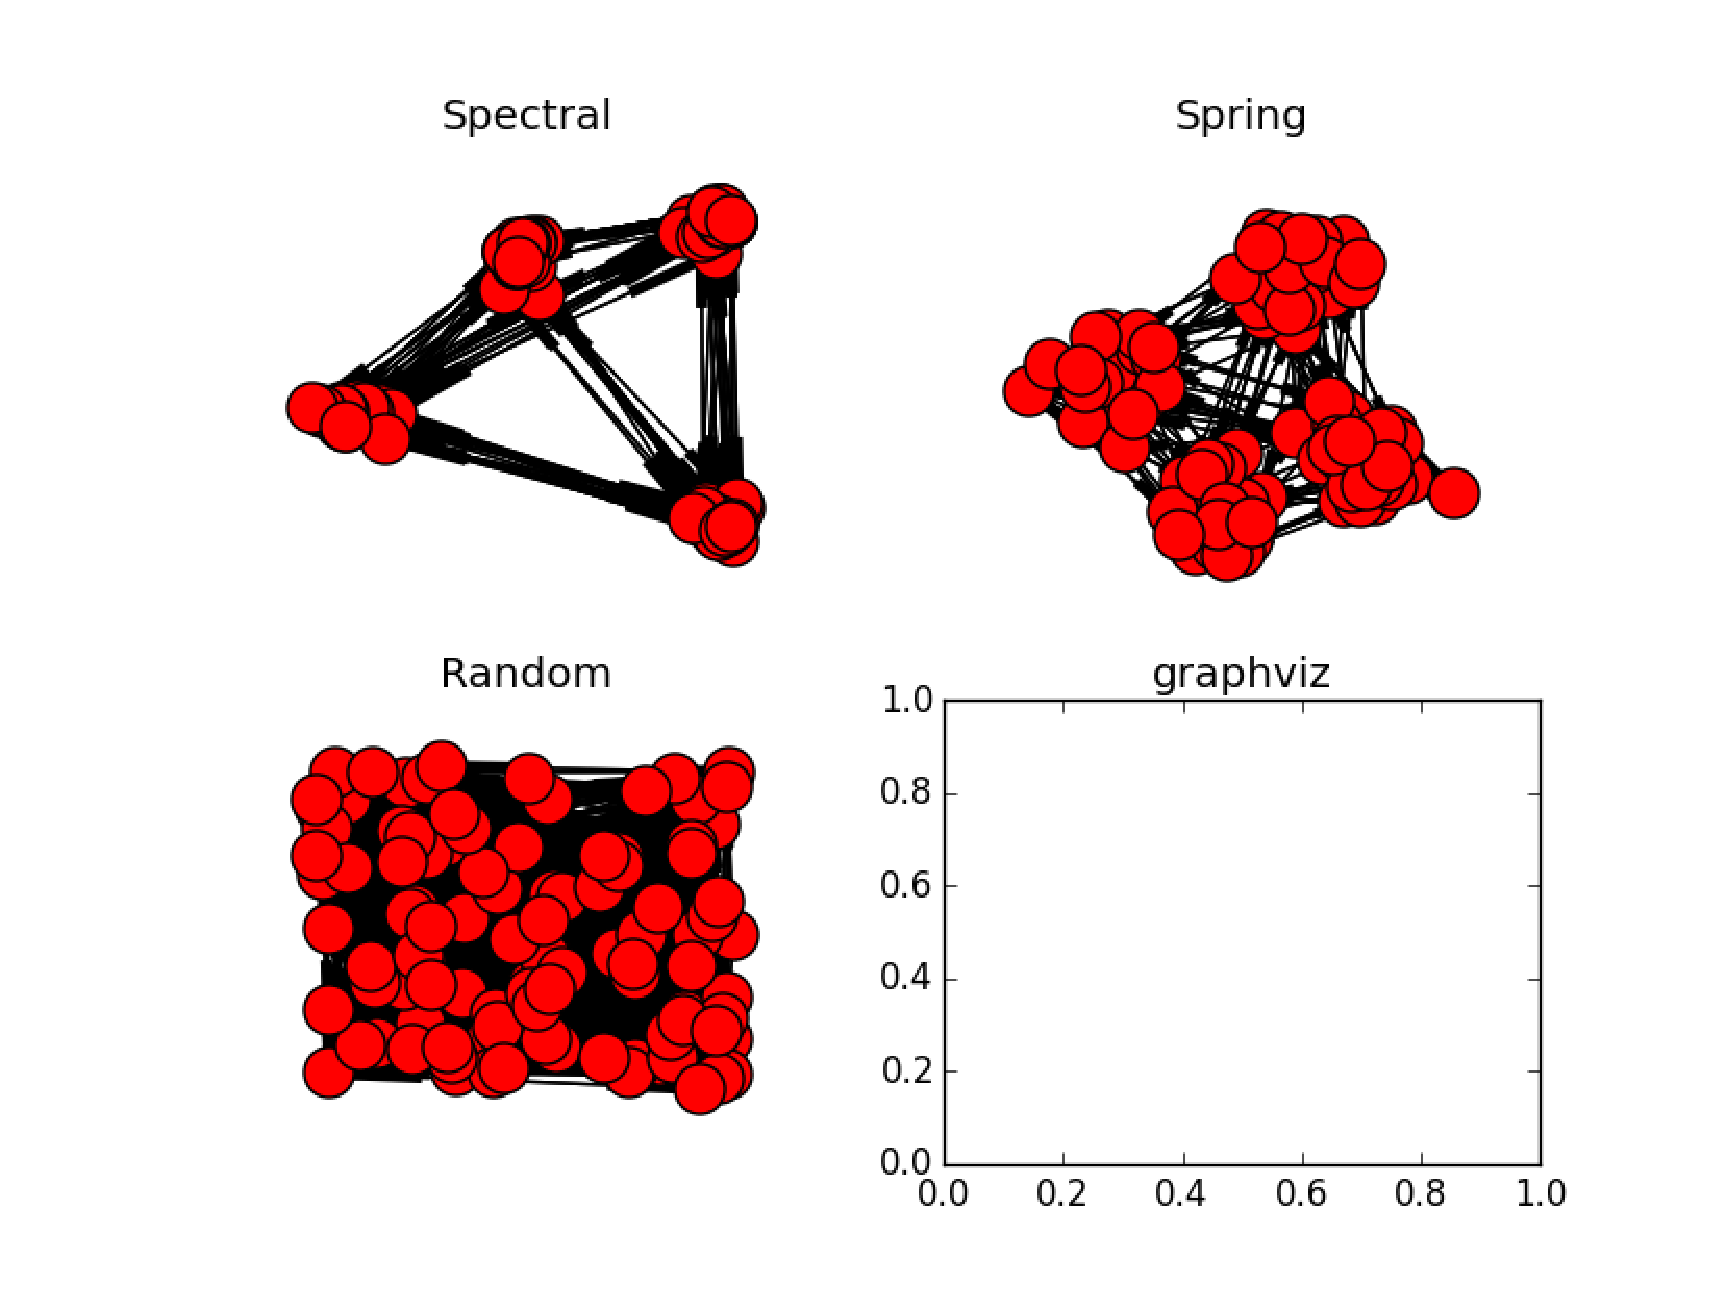
\includegraphics[scale=0.3]{img/networks}
    \end{figure}
\end{frame}

\begin{frame}[c]{Social Networks Properties}
    \textit{\Large{Important properties observed in social networks}}
    \vspace{2em}

\scalebox{0.82}{
    {\renewcommand{\arraystretch}{1.8}
    \begin{tabular}{|c|c|}
    \hline
    \textbf{Property} & \textbf{Measure} \\
    \hline
    \hline
    Small World & Diameter  (Millgram 1978, Leskovec 2008 )\\
    \hline
    Community & Modularity, Clustering Coefficient (Newman 2006) \\
    \hline
    Homophily & Homophily Coefficient (McPherson 2001, Kleinberg 2010) \\
    \hline
    Preferential Attachment / Burstiness & Degree Distribution (Barab\'asi 1999) \\
    \hline
    Sparsity & Density (Haldous, Hoover 1981) \\
    \hline
    \end{tabular}}
    }
\end{frame}


%
%
% Why probabilistic models.
% (who use it, why)
%
%

\begin{frame}[t]{Statement}
    \vspace{3em}

    \textit{\Large{We focus on two models in the class of Mixed-Membership Models: }}
    \begin{itemize}
        \item IMMSB (Infinite Mixed-Membership Stochastic Blockmodel)
        \item ILFM (Infinite Latent Feature Model) 
    \end{itemize}

    \vspace{2em}

    \textit{\Large{Do those models comply with preferential attachment?}}\\
    \vspace{1em}
    \textit{\Large{homophily?}}\\
    \vspace{1em}
    \textit{\Large{What is the impact?}}


\pause

\begin{block}{Claims}
\begin{tabular}{l|cc|c}

        \multicolumn{3}{c}{\hspace{1.3cm}\textbf{Preferential Attachment}}   \\
        \cmidrule(l){2-3} 
        &   global & local  &   \textbf{homophily}      \\
        \hline
        ILFM       & \cellcolor{red!25}No & \cellcolor{red!25}No   & depends on similarity  \\
        IMMSB       & \cellcolor{red!25}No & \cellcolor{green!25}Yes  & depends on similarity \\
    \end{tabular}
\end{block}

\end{frame}

\section{Probabilistic Graph Models}

%
% People like it 
%

\begin{frame}[t]{Probabilistic Model}

    % digression for recall on probabilistic modeling and bayesian reasoning

    \begin{columns}[t]
    \begin{column}{0.8\textwidth}
    \begin{block}{The Joint Distribution}
        $P(Y,\Theta \mid\sigma)$: How observations of a natural phenomena arise
    \end{block}

    \begin{block}{Likelihood}
        $P(Y \mid \Theta)$: How observations depend on the latent variables
    \end{block}

    \begin{block}{Prior}
        $P(\Theta \mid\sigma)$: Describe the latent variables of the model
    \end{block}

    \end{column}
    \begin{column}{0.25\textwidth}

        \begin{block}{Graphical Model}
            \centering
            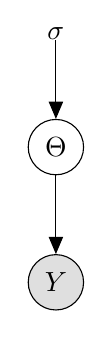
\begin{tikzpicture}
                \node[const] (a) {$\sigma$};
                \node[latent, below=of a] (p) {$\Theta$};
                \node[obs, below=of p] (y) {$Y$};

                \edge {a}{p};
                \edge {p}{y};
            \end{tikzpicture}

        \end{block}
    \end{column}
    \end{columns}

    \pause

    \begin{columns}[t]
        \begin{column}{0.35\textwidth}
        \begin{block}{The generative process}
            \begin{align*}
                \Theta &\sim P(\Theta \mid \sigma) \\
                y &\sim P(y \mid\Theta)
            \end{align*}
        \end{block}
        \end{column}
        \begin{column}{0.65\textwidth}
        \begin{block}{Inference / Optimisation}
            Posterior Distribution: $\textcolor{blue}{P(\Theta \mid Y)}  = \frac{P(Y|\Theta)P(\Theta)}{P(Y)}$
        \end{block}
        \end{column}
    \end{columns}

\end{frame}


%\begin{frame}[c]{Predictions}
%    Predictions involve the posterior distribution (+ sum and product rules):
%
%    \begin{align}
%        p(y^{new}| Y, \sigma) &= \int_\Theta P(y^{new}|\Theta) \textcolor{blue}{P(\Theta | Y, \sigma)}\ d\Theta \\
%                              &= \mathbb{E}_{\Theta \sim P(\Theta | Y, \sigma)} [P(y^{new}|\Theta)]
%    \end{align}
%
%    \underline{\alert{NOTE}}: Assumption of conditional independancy of observations in the likelihood. (Static Networks)
%    
%\end{frame}

%\begin{frame}[t]{Regression Example (Ridge)}
%
%    Given $Y$ and $X$:
%
%    \begin{equation*}
%        Y_i = \sum_k x_k \beta_k + \varepsilon_i  \qquad (\textrm{matrix form}: Y = \bm{\beta}^T X + \mathcal{E} )
%    \end{equation*}
%
%    Find $\bm{\beta}$ ?
%
%    \pause
%
%    \begin{columns}[t]
%        \begin{column}{0.4\textwidth}
%            \vspace{-2cm}
%            \begin{align*}
%                \beta_k &\sim \mathcal{N}(0, \sigma) \\%= \frac{1}{\sqrt{2\pi\sigma }}e^{-\frac{\beta_k^2}{2\sigma}} \\
%                y_i &\sim \mathcal{N}(\beta^T X_i, \sigma_n) 
%            \end{align*}
%            \vfill
%        \end{column}
%        \begin{column}{0.5\textwidth}
%            \begin{tikzpicture}
%                \node[obs, below=of p] (y) {$Y_i$};
%                \node[obs, left=of y] (x) {$X_i$};
%                \node[latent, right=of y] (p) {$\beta_k$};
%                \node[const, above=of p] (a) {$\sigma$};
%                \node[const, above=of y] (n) {$\sigma_n$};
%
%                \edge {a}{p};
%                \edge {p}{y};
%                \edge {x}{y};
%                \edge {n}{y};
%
%                \plate {} {(x)(y)} {$N$} ;
%                \plate {} {(p)} {$K$} ;
%            \end{tikzpicture}
%
%        \end{column}
%    \end{columns}
%
%    \pause
%
%    Optimisation Problem: 
%    \begin{align*}
%        \mathrm{arg}\max\limits_{\bm{\beta}}  P(\bm{\beta}| Y, X) &= P(Y | \bm{\beta}, X) P(\bm{\beta}) \\
%        &=  \prod_i P(Y_i | \beta,  X_i) \prod_k P(\beta_k) \\
%        \mathrm{arg}\min\limits_{\bm{\beta}}  -\log(P(\bm{\beta}| Y, X))  &=  \sum_i (Y_i - \bm{\beta}^T X_i)^2  + \frac{\sigma_n}{\sigma}\sum_k \beta_k^2
%    \end{align*}
%
%\end{frame}


\begin{frame}[t]{Social Network to Graph}

    %Graph and adjacency matrix define the topology of a network.

    \begin{description}[align]
        \item[A graph]: $G = (V,E)$
            \begin{itemize}
                \item $V$: set of vertices, drawn as nodes,
                \item $E$: set of edges, drawn as lines connecting vertices,
            \end{itemize}

        \item[containing $N$ nodes]:  $|V| = N$
        \item[Define a adjacency matrix]:  $Y=(y_{ij})_{i,j \in V^2} \left| \substack{\ y_{ij}=1 \quad \textrm{if } (i,j) \in E \\ \ y_{ij}=0 \quad \textrm{otherwise} } \right.\kern-\nulldelimiterspace  $
    \end{description}

    \begin{columns}
        \begin{column}{0.5\textwidth}
        \begin{figure}[h]
        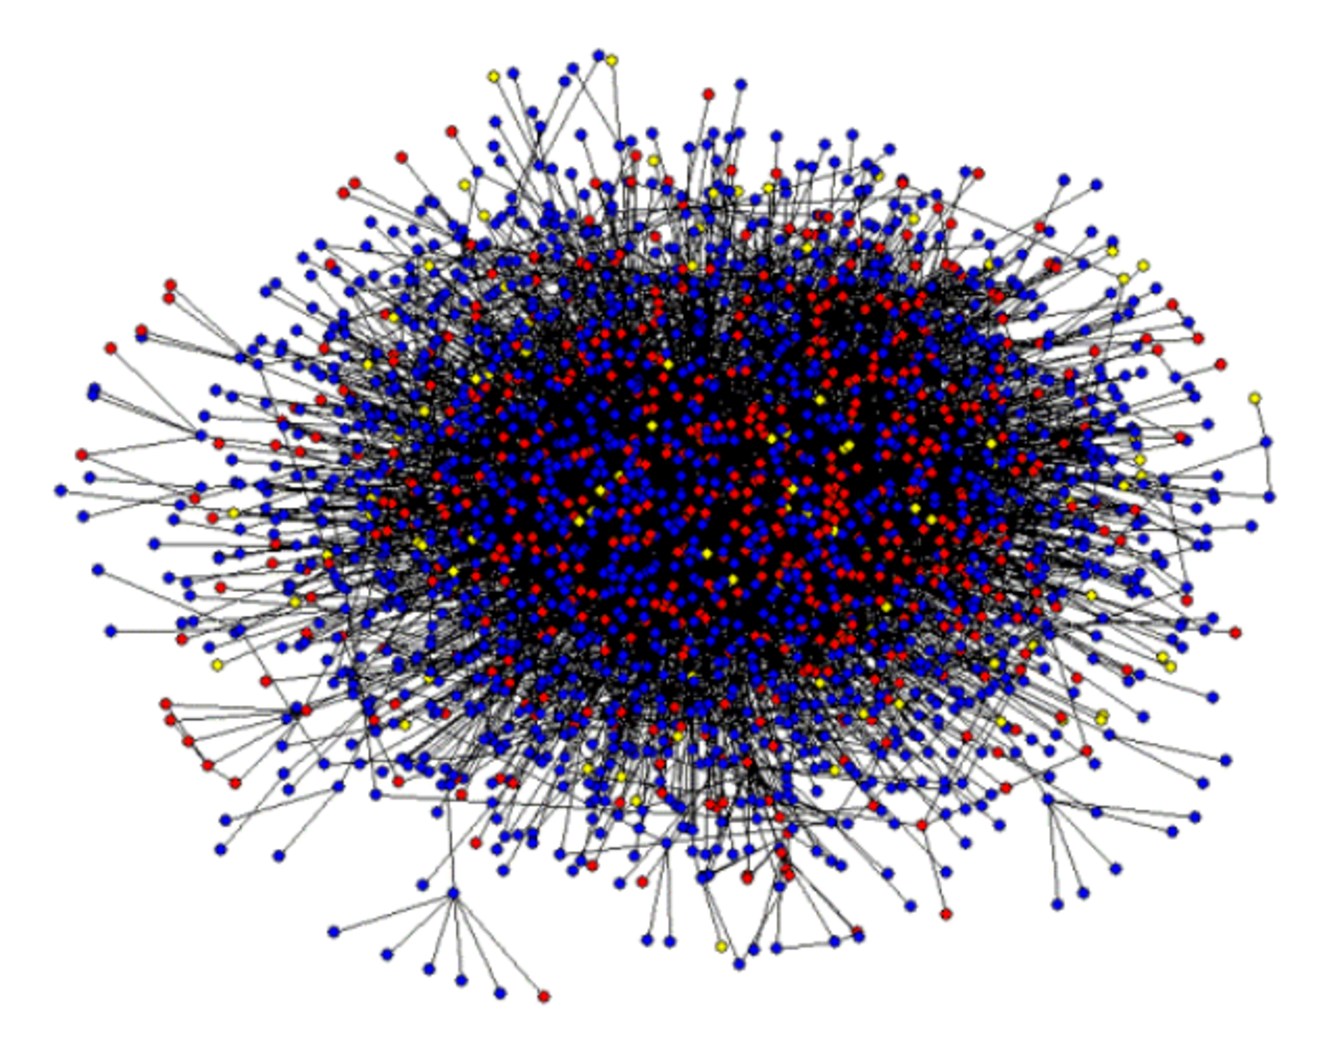
\includegraphics[scale=0.25]{img/net.pdf}
        \end{figure}
        \end{column}
        \begin{column}{0.5\textwidth}
        \begin{figure}[h]
        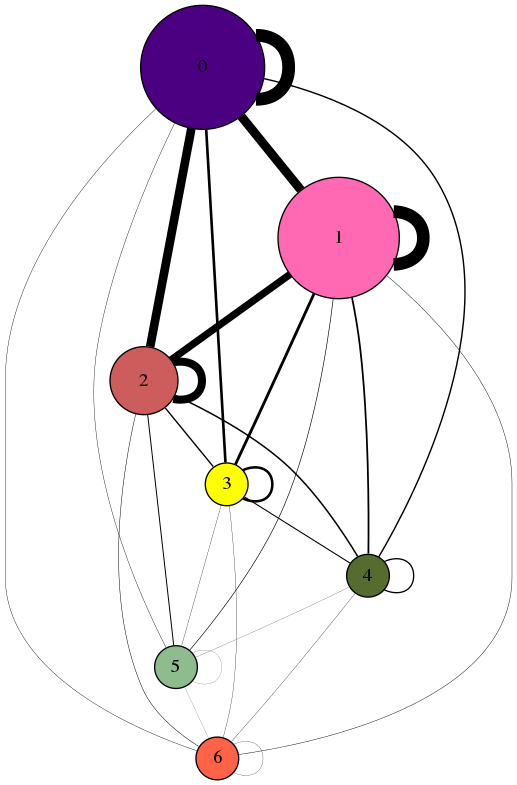
\includegraphics[scale=0.15]{img/gdot.png}
        \end{figure}
        \end{column}
    \end{columns}
\end{frame}

%
%
% Insist on reading the matrix to the graph (it helps)
%
%




\begin{frame}[t]{Random Graph model}

Given a Graph $G=(V,E)$,  we define $\textcolor{blue}{F}$ and $\textcolor{green}{\Phi}$ such that:

\begin{equation*}
    Y \sim P(Y | \textcolor{blue}{F}, \textcolor{green}{\Phi}) =h( \textcolor{blue}{F}\textcolor{green}{\Phi} \textcolor{blue}{F}^T )
\end{equation*}


\begin{description}
\setlength{\itemindent}{-2cm}
\item[\textcolor{blue}{$F$}]: a latent feature matrix (describes the membership of nodes)
\item[\textcolor{green}{$\Phi$}]: a latent weight matrix (describes the correlation between classes)
\item[$h$]: a mapping function to a probability space.
\end{description}

\pause


    \begin{columns}
        \begin{column}{0.6\textwidth}
            
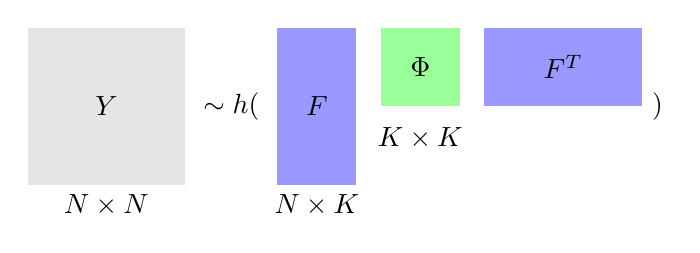
\begin{tikzpicture}[scale=.5]



\node (y) [rectangle, fill=black!10, minimum height=2cm, minimum width=2cm] {$Y$};
    \node (eq) [right=0.1cm of y] {$\sim h($};
\node (p) [rectangle, fill=blue!40, minimum height=2cm, minimum width=1cm, right=0.1cm of eq] {$F$};
\node (f) [rectangle, fill=green!40, minimum height=1cm, minimum width=1cm, yshift=0.5cm , right=0.3cm of p] {$\Phi$};
\node (pt) [rectangle, fill=blue!40, minimum height=1cm, minimum width=2cm,  right=0.3cm of f] {$F^T$};
    \node (close) [yshift=-0.5cm, right=0cm of pt] {)};

\node[below of=y, yshift=-0.25cm] (Y) {$N \times N$};
\node (F) [below of=p, yshift=-0.25cm] {$N \times K$};
\node (P) [below of=f, yshift=0.1cm] {$K \times K$};


\end{tikzpicture}



    \begin{block}{Likelihood}
    \[ P(y_{ij}=1 | F, \Phi) = h(f_i \Phi f_j^T) \]
    \end{block}
    What prior over $F$ and $\Phi$ ?
        \end{column}
        \begin{column}{0.4\textwidth}
        \begin{figure}[h]
        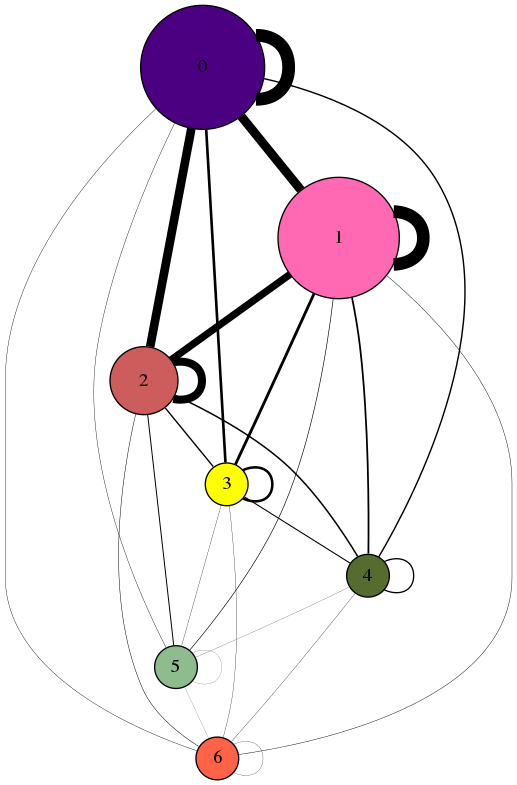
\includegraphics[scale=0.15]{img/gdot.png}
        \end{figure}
        \end{column}
    \end{columns}


\end{frame}

\newcounter{row}
\newcounter{col}
\newcommand\setrow{}

\begin{frame}[t]{Stochastic Blockmodel}
    The Stochastic Blockmodel \footfullcite{goldenberg2010survey}

    \begin{itemize}
        \item We have $K$ blocks
        \item Any node $i$ belongs to only one block $c$
        \item Each weight $(\phi_{kl})_{k,l \in (1, .., K)^2}$ ,  encodes the strength between two blocks.
    \end{itemize}

    \vspace{1em}
    \emph{One Example:}

    \begin{block}{Block membership for node 4 and 7 (K=3 and N=9)}

    \begin{columns}[t]
        \begin{column}{0.45\textwidth}
        $f_4$ = \raisebox{-2pt}{%\newcounter{row}
%\newcounter{col}
\setcounter{row}{0}
\setcounter{col}{0}

\renewcommand\setrow[3]{
    \setcounter{col}{1}
    \foreach \n in {#1, #2, #3} {
        \edef\x{\value{col} -0.5}
        \edef\y{\value{row} -0.5}
        \node[anchor=center] at (\x, \y) {\n};
        \stepcounter{col}
    }
    \stepcounter{row}
}

\begin{tikzpicture}[scale=.5]

    \begin{scope}
        \draw (0, 0) grid (3, 1);
        %\draw[very thick, scale=3] (0, 0) grid (3, 3);

    \setcounter{row}{1}
        \setrow {0}{1}{0}  {0}{0}

        %\node[anchor=center] at (4.5, -0.5) {};
    \end{scope}
\end{tikzpicture}
}
        \end{column}
        \begin{column}{0.45\textwidth}
            \hspace{-1.5cm}
        $f_7$ = \raisebox{-2pt}{%\newcounter{row}
%\newcounter{col}
\setcounter{row}{0}
\setcounter{col}{0}

\renewcommand\setrow[3]{
    \setcounter{col}{1}
    \foreach \n in {#1, #2, #3} {
        \edef\x{\value{col} -0.5}
        \edef\y{\value{row} -0.5}
        \node[anchor=center] at (\x, \y) {\n};
        \stepcounter{col}
    }
    \stepcounter{row}
}

\begin{tikzpicture}[scale=.5]

    \begin{scope}
        \draw (0, 0) grid (3, 1);
        %\draw[very thick, scale=3] (0, 0) grid (3, 3);

    \setcounter{row}{1}
        \setrow {0}{0}{1}  

        %\node[anchor=center] at (4.5, -0.5) {};
    \end{scope}
\end{tikzpicture}
}
            \hspace{0.5cm}
        $\phi_{12} = 0.3$
        \end{column}
    \end{columns}

    \end{block}

    \begin{figure}[h]
    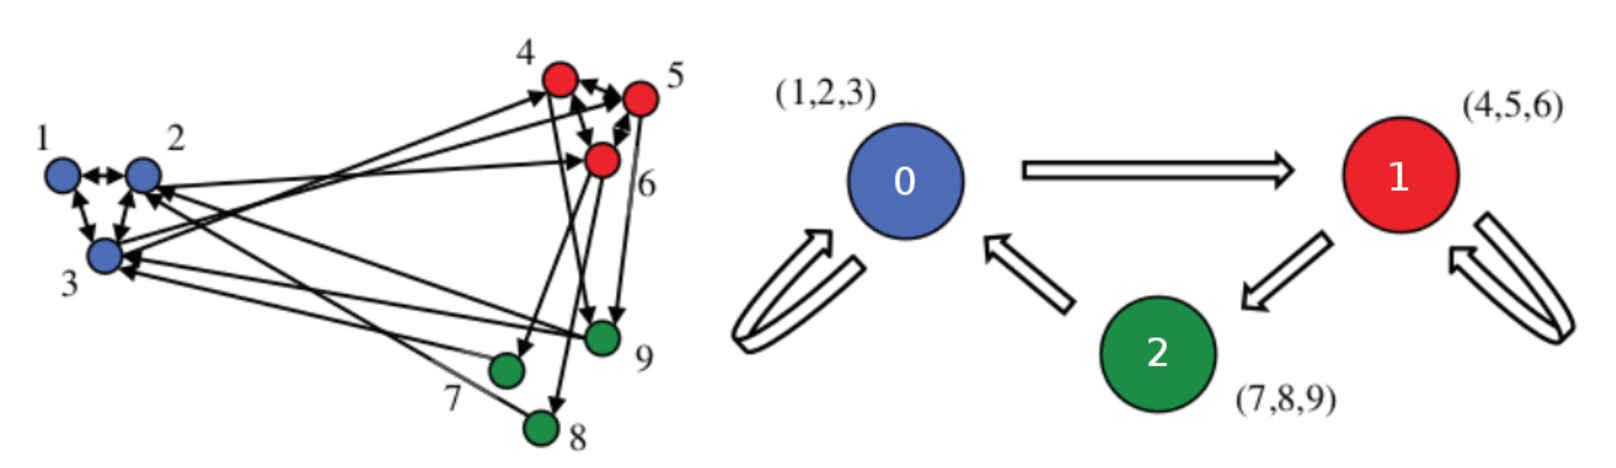
\includegraphics[scale=0.3]{img/sb}
        \caption{Stochastic Blockmodel}
    \end{figure}
    
\end{frame}

\begin{frame}[c]{Mixed Membership Models}

    Relax the single membership assumption (soft clustering).

    \begin{block}{Binary features (ILFM)}
        $f_i$ = \raisebox{-2pt}{%\newcounter{row}
%\newcounter{col}
\setcounter{row}{0}
\setcounter{col}{0}

\renewcommand\setrow[5]{
    \setcounter{col}{1}
    \foreach \n in {#1, #2, #3, #4, #5} {
        \edef\x{\value{col}*1.2 -0.5*1.2}
        \edef\y{\value{row} -0.5}
        \node[anchor=center] at (\x, \y) {\n};
        \stepcounter{col}
    }
    \stepcounter{row}
}

\begin{tikzpicture}[scale=.5]

    \begin{scope}
        \draw[xscale=1.2] (0, 0) grid (5, 1);
        %\draw[very thick, scale=3] (0, 0) grid (3, 3);

    \setcounter{row}{1}
        \setrow {1}{0}{1}{1}{0}

        %\node[anchor=center] at (4.5, -0.5) {};
    \end{scope}
\end{tikzpicture}
}
    \end{block}
    ILFM relax the fixed number of features $K$ with an Indian Buffet Process (IBP). \\
    %And Gaussian weights...

    \vspace{0.2cm}
    \emph{or}
    \vspace{0.2cm}

    \begin{block}{Proportion features (MMSB)}
        $f_i$ = \raisebox{-2pt}{%\newcounter{row}
%\newcounter{col}
\setcounter{row}{0}
\setcounter{col}{0}

\renewcommand\setrow[5]{
    \setcounter{col}{1}
    \foreach \n in {#1, #2, #3, #4, #5} {
        \edef\x{\value{col}*1.2 -0.5*1.2}
        \edef\y{\value{row} -0.5}
        \node[anchor=center] at (\x, \y) {\n};
        \stepcounter{col}
    }
    \stepcounter{row}
}

\begin{tikzpicture}[scale=.5]

    \begin{scope}
        \draw[xscale=1.2] (0, 0) grid (5, 1);
        %\draw[very thick, scale=3] (0, 0) grid (3, 3);

    \setcounter{row}{1}
        \setrow {.5}{.2}{.1}{.1}{.1}

        %\node[anchor=center] at (4.5, -0.5) {};
    \end{scope}
\end{tikzpicture}
} \hspace{2em} $\sum f_i=1$
    \end{block}
    IMMSB also relax the fixed number of features $K$ with a (Hierarchical) Dirichlet Process (DP). \\
    %And beta weights...
    
\end{frame}

\begin{frame}[c]{IMMSB}

    Infinite Mixed Membership Stochastic Model (IMMSB) \footfullcite{IMMSB}
    \vspace{1cm}

    \begin{columns}[t]
        \begin{column}{0.5\textwidth}
            \vspace{-5cm}
            \begin{align*}
                &\bm{\beta} \sim \textrm{GEM}(\gamma)\\
                &\textrm{For each } i \in \{1, .., N\}  \\
                &\qquad\bm{f}_i \sim \textrm{DP}(\alpha_0, \bm{\beta})\\
                &\textrm{For each }  (m,n) \in \{1,..,K\}^2 \\
                &\qquad\phi_{mn} \sim \mathrm{Beta}(\lambda_0,\lambda_1)\\
                &\textrm{For each } (i,j) \in V^2 \\
                &\qquad z_{i \rightarrow j} \sim \mbox{Mult}(\bm{f}_i)\\
                &\qquad z_{i \leftarrow j} \sim \mbox{Mult}(\bm{f}_j)\\
                &\qquad y_{ij} \sim \mathrm{Bern}({z_{i \rightarrow j} \Phi z_{i \leftarrow j}^T})
            \end{align*}
        \end{column}
        \begin{column}{0.5\textwidth}
            \scalebox{0.88}{/home/dulac/Documents/workInProgress/networkofgraphs/papers/personal/figures/draw/mmsb2.tex}
        \end{column}
    \end{columns}

\end{frame}

\begin{frame}[c]{ILFM}

    Infinite Latent Feature Model (ILFM) \footfullcite{ILFRM}
    \vspace{1cm}

    \begin{columns}[t]
        \begin{column}{0.5\textwidth}
            \vspace{-4cm}
            \begin{align*}
                &F \sim \textrm{IBP}(\alpha)\\
                &\textrm{For each }  (m,n) \in \{1,..,K\}^2 \\
                &\qquad\phi_{mn} \sim \mathrm{Gaussian}(0,\sigma_w)\\
                &\textrm{For each } (i,j) \in V^2 \\
                &\qquad y_{ij} \sim \mathrm{Bern}(\bm{f}_i \Phi \bm{f}_j^T)
            \end{align*}
        \end{column}
        \begin{column}{0.5\textwidth}
            \scalebox{0.88}{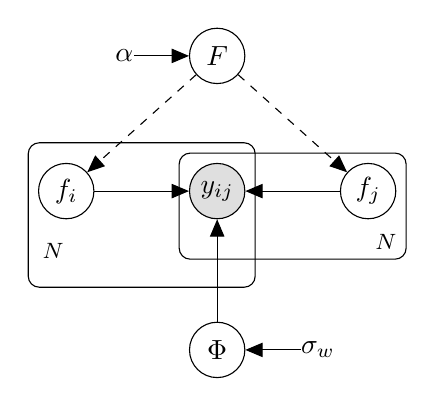
\begin{tikzpicture}
  % Define nodes
  \node[obs]                      (y) {$y_{ij}$};
  \node[latent, left=1.2cm of y] (fi) {$\mat{f}_i$};
  \node[latent, right=1.2cm of y] (fj) {$\mat{f}_j$};
  \node[latent, above= of y]    (ibp) {$\mat{F}$};;
  \node[latent, below= of y, yshift=-0.3cm]   (W) {$\mat{\Phi}$};
  \node[const, left=0.7cm of ibp]   (a) {$\alpha$};
  \node[const, right=0.7cm of W]   (sw) {$\sigma_w$};

  % Connect the nodes
  \edge {fi,fj,W} {y} ;
  \edge[dashed] {ibp} {fi,fj} ;
  \edge {sw} {W} ; 
  \edge {a} {ibp} ; 

  % Plates
  \plate {yx} {(fj)(y)} {$N$} ;
  \plate[label={[label distance=-0.6cm]195:$N$}] {} {(fi)(y)(yx.north west)(yx.south west)} {} ;
  %\plate {} {(W)} {$K\times K$};
  %\plate {} {(fi)(y)(yx.north west)(yx.south west)} {$N$} ;
\end{tikzpicture}
}
        \end{column}
    \end{columns}
\end{frame}

\section{Properties Characterization}


\begin{frame}[c]{Preferential attachment}


    \begin{definition}[Degrees]
    Let $\mathcal{M}_e = \{ \textcolor{blue}{F}, \textcolor{green}{\Phi} \}$ be a probabilistic link prediction model such that 
    \[Y\sim P(Y|\mathcal{M}_e) \]

    Let $\mathcal{C}_k$ be the set of nodes belonging to the class $k$ such that
    \[\mathcal{C}_k\sim P(\mathcal{C}_k|\mathcal{M}_e) \]

    \begin{itemize}
    \item Global degree : $d_i  = \sum_{j\neq i} y_{ij}$
    %\item Local degree :  $d_{ik}  = \sum_{j\neq i} y_{ij} \mathbbm{1}(i,j\in \mathcal{C}_k)$
    %\item Expected Local degree :  $D_{ik}  = \sum_{j\neq i} P(y_{ij}=1, i,j\in \mathcal{C}_k | \mathcal{M}_e) $
    \item  Local degree :  $d_{i,k}  = \sum_{j\neq i} P(y_{ij}=1, i,j\in \mathcal{C}_k | \mathcal{M}_e) $
    \end{itemize}
    \end{definition}

    %Note: In practice, class are not directly observed, thus we have to resort to the the expected local degree.
    %
    % I don't like this assertion, still its incorecct, membership for ILFM are hard and
    % Known given F. For MMSB, it can be says tough the membership are not direcly
    % observed stil it's an expection over the Z.
    %



    % Power law figure on real dataset...
    %\begin{figure}[h]
    %    \caption{power law distribution in real datasets}
    %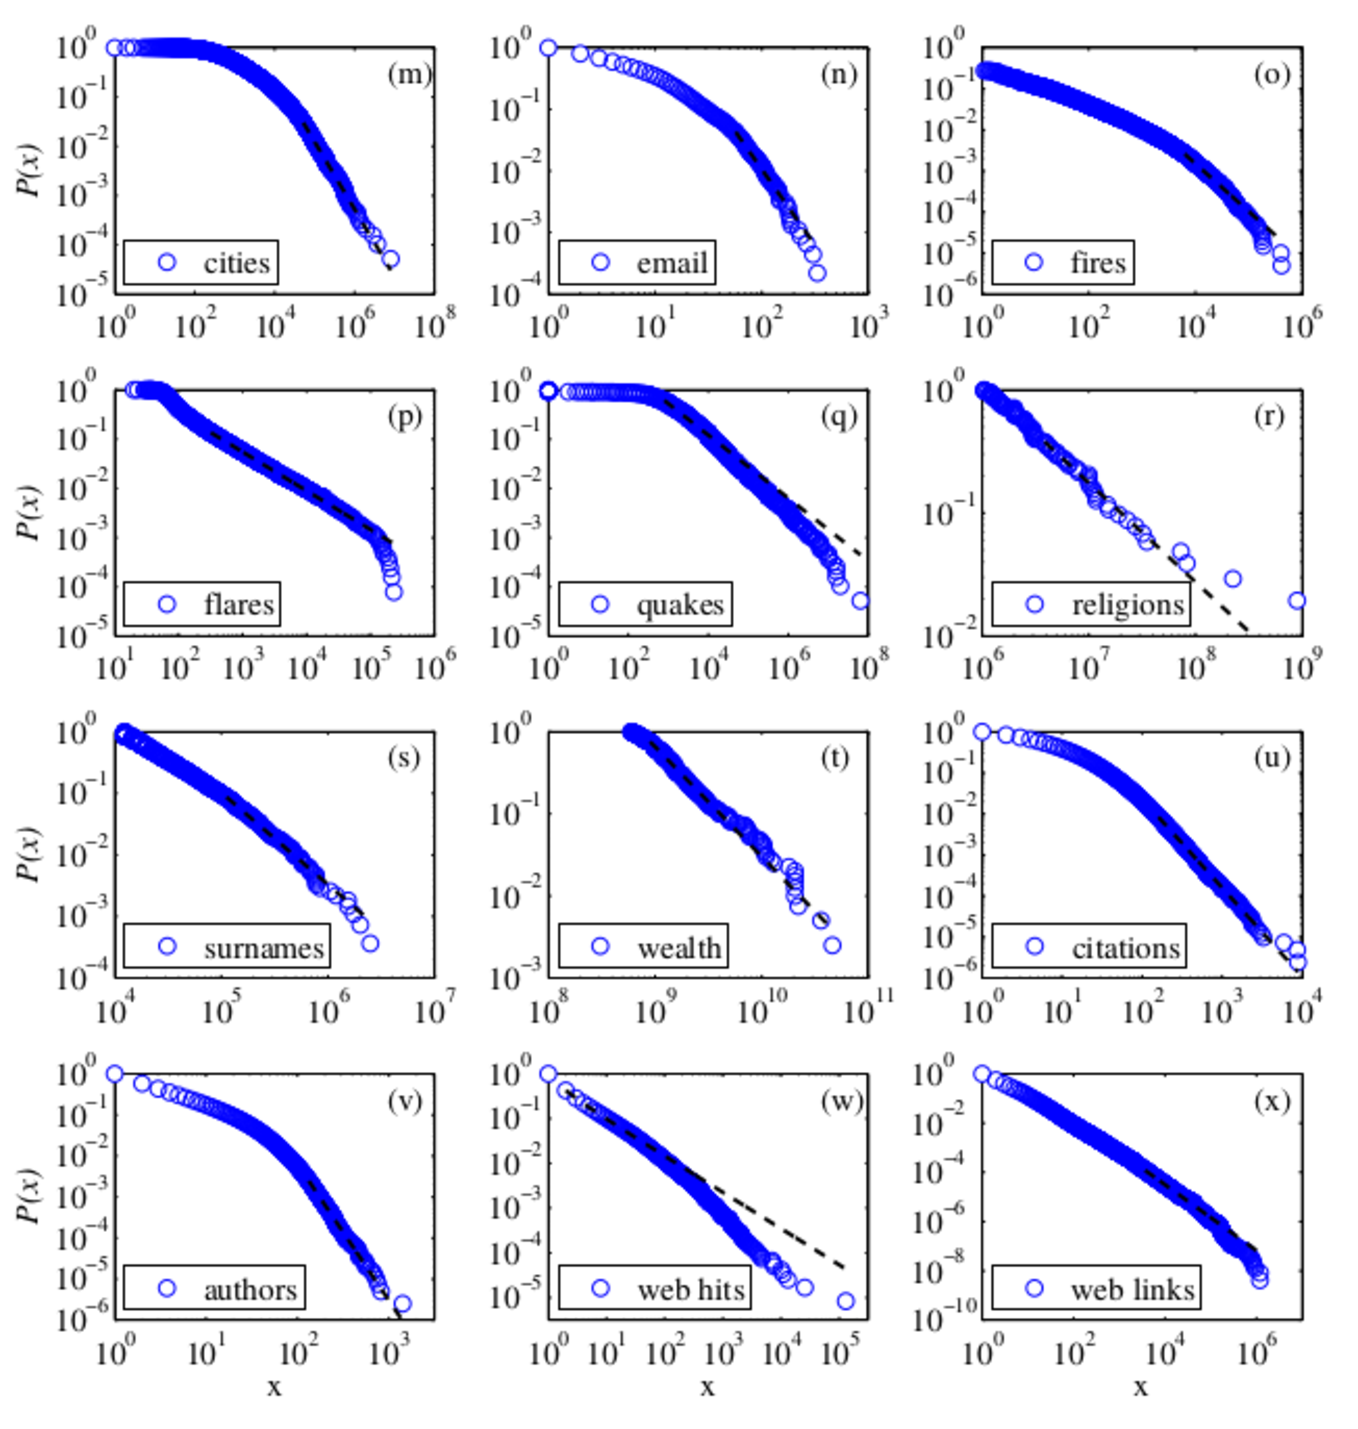
\includegraphics[width=7cm, height=5.1cm]{img/power_law.pdf}
    %\end{figure}
    %\footfullcite{clauset2009power}

\end{frame}


\begin{frame}[c]{Preferential attachment (cont.)}

\emph{The rich get richer...}
\vspace{2em}

\begin{definition}[Global Preferential attachment]
we say that $\mathcal{M}_e$ satisfies the global preferential attachment iff, for any node $i$, 
\[P(d_i \ge n+1 \mid d_i \ge n, \mathcal{M}_e) \textrm{ increases with } n \in \{0,..., N-2\} \]
\end{definition}

\begin{definition}[Local Preferential attachment]
we say that  $\mathcal{M}_e$ satisfies the local preferential attachment iff, for any node $i$, 
\[P(d_{i,k} \ge x+\epsilon \mid d_{i,k} \ge x, \mathcal{M}_e) \textrm{ increases with } x \in [0,N[ \]
\end{definition}

\end{frame}

\begin{frame}[c]{Preferential attachment (cont.)}

\begin{block}{Proposition (Global preferential attachment)}
Both IMMSB and ILFM  do not satisfy global preferential attachment.
\end{block}
Clue =$>$ \underline{Exchangeability}

\vspace{1em}

\begin{block}{Proposition (Local preferential attachment)}
IMMSB satisfies local preferential attachment whereas ILFM does not.
\end{block}
Clue =$>$ \underline{Conjugacy}

\end{frame}


\begin{frame}[c]{Homophily}

\emph{Birds of a feather flock together...}
\vspace{2em}

\begin{definition}[Homophily]
Let $s$ be a similarity measure between nodes. 
We say that $\mathcal{M}_e$ is homophilic under the similarity $s$ iff, $\forall (i,j,i',j') \in V^4$:

\[ s(i,j) > s(i',j')  \implies P(y_{ij}=1 \mid \mathcal{M}_e) > P(y_{i'j'}=1  \mid \mathcal{M}_e) \]

\end{definition}

\begin{block}{Similarities}
    \begin{description}
    \item[Natural similariry] : $s_n = f_i \Phi f_j\top $
    \item[Latent similarity] \ : $s_l = f_i f_j^\top$
    \end{description} 
\end{block}

\end{frame}

\begin{frame}{Homophily (cont.)}

\begin{block}{Proposition (Homophily with $s_n$)}
Both IMMSB and ILFM are homophilic with respect to the natural similarity $s_n$.
\end{block}

\vspace{2em}

\begin{block}{Proposition (Homophily with $s_l$)}
Neither IMMSB nor ILFM are homophilic with respect to the latent similarity $s_l$.
\end{block}

\end{frame}



\section{Illustrations}

\begin{frame}[c]{Theoretical Results}

    Summary of our theoretical results. %\footfullcite{A study of stochastic mixed membership models for link prediction in social networks: Under Revision}
    \vspace{1cm}


    \begin{block}{Theoretical results}
	\begin{tabular}{l|cc|c}

        \multicolumn{3}{c}{\hspace{1.3cm}\textbf{Preferential Attachment}}   \\
        \cmidrule(l){2-3} 
        &   global & local  &   \textbf{homophily}      \\
        \hline
        ILFM       & \cellcolor{red!25}No & \cellcolor{red!25}No   & depends on similarity  \\
        IMMSB       & \cellcolor{red!25}No & \cellcolor{green!25}Yes  & depends on similarity \\
    \end{tabular}

    \end{block}

\end{frame}

\begin{frame}[c]{Empirical Results (Datasets)}

    \vspace{-0.2cm}
\begin{table}[h] 
	\centering
	\caption{Characteristics of artificial and real networks.}
    \begin{tabular}{lrrr}
        \hline
        \textbf{Networks} &   nodes &   edges &   density \\
        \hline
        Network1 &    1000 &    3507 &     0.007 \\
        Network2 &    1000 &   31000 &     0.062 \\
        Blogs         &    1490 &   20512 &     0.009 \\
        Manufacturing &     167 &    5950 &     0.215 \\
    \hline
    \end{tabular}
	\label{table:networks_measures}
\end{table}

\begin{table}[t]
\caption{Preferential attachment measures for training datasets and networks generated with fitted models.}
\centering
\begin{tabular}{lrrrr}
  \multirow{2}{*}{\textbf{Training Datasets}}  &
  \multicolumn{2}{c}{Global} & \multicolumn{2}{c}{Local}\\
  \cmidrule(r){2-3} \cmidrule(l){4-5}
  &   $p$-value &   $\alpha$   & $p$-value & $\alpha$   \\
\hline
Network1       & 1 & 2.4 &   1.0 $\pm$ 0.0  &  1.8 $\pm$ 0.03  \\
Network2       & 0 & 1.3 &   0.0 $\pm$ 0.0  &  1.2 $\pm$ 0.01 \\
Blogs          & 1 & 1.5 &   1.0 $\pm$ 0.0  &  1.4 $\pm$ 0.03\\
Manufacturing  & 0 & 1.4 &   0.4 $\pm$ 0.3  &  1.3 $\pm$ 0.05 \\
\hline
\end{tabular}
\label{table:me_gofit}
\end{table}

\end{frame}


\begin{frame}[c]{Empirical Results (Preferential attachment I)}

    \vspace{-0.2cm}

    \begin{columns}[t]
        \begin{column}{0.5\textwidth}
        \begin{figure}[h]
            \caption{Synthetic Datasets}
        %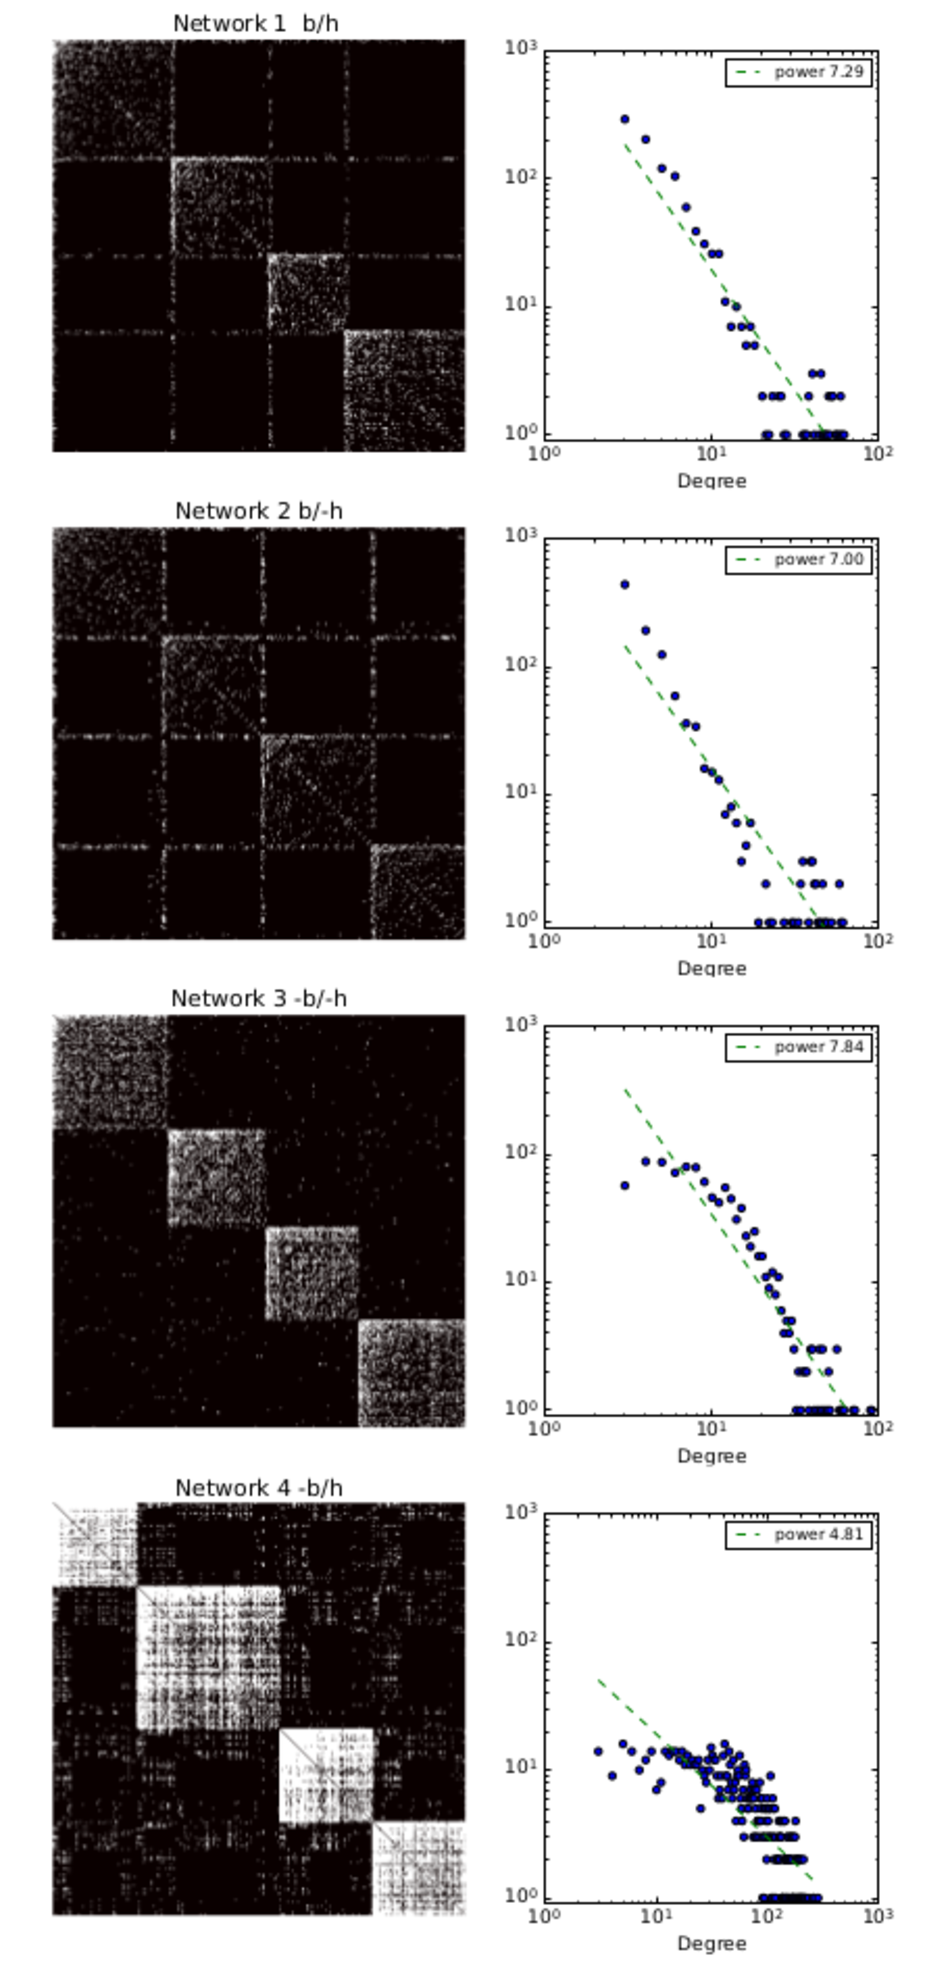
\includegraphics[scale=0.2]{img/burst_sint.pdf}
        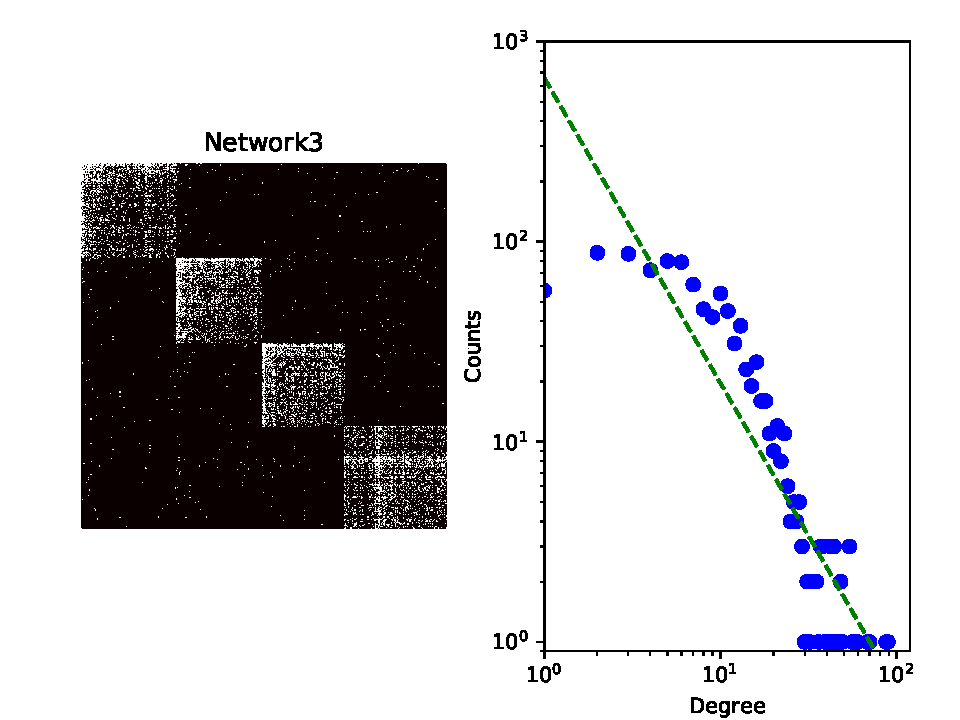
\includegraphics[scale=0.28]{img/Network3_0.pdf}
        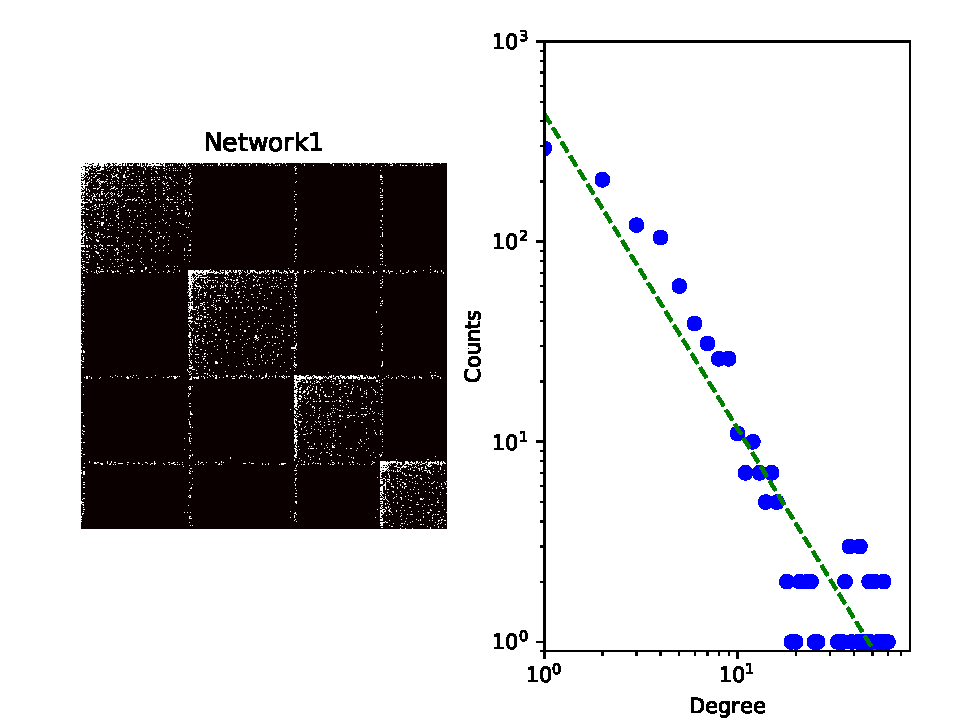
\includegraphics[scale=0.28]{img/Network1_0.pdf}
        \end{figure}
        \end{column}
        \begin{column}{0.5\textwidth}
        \begin{figure}[h]
            \caption{Prediction Performance}
        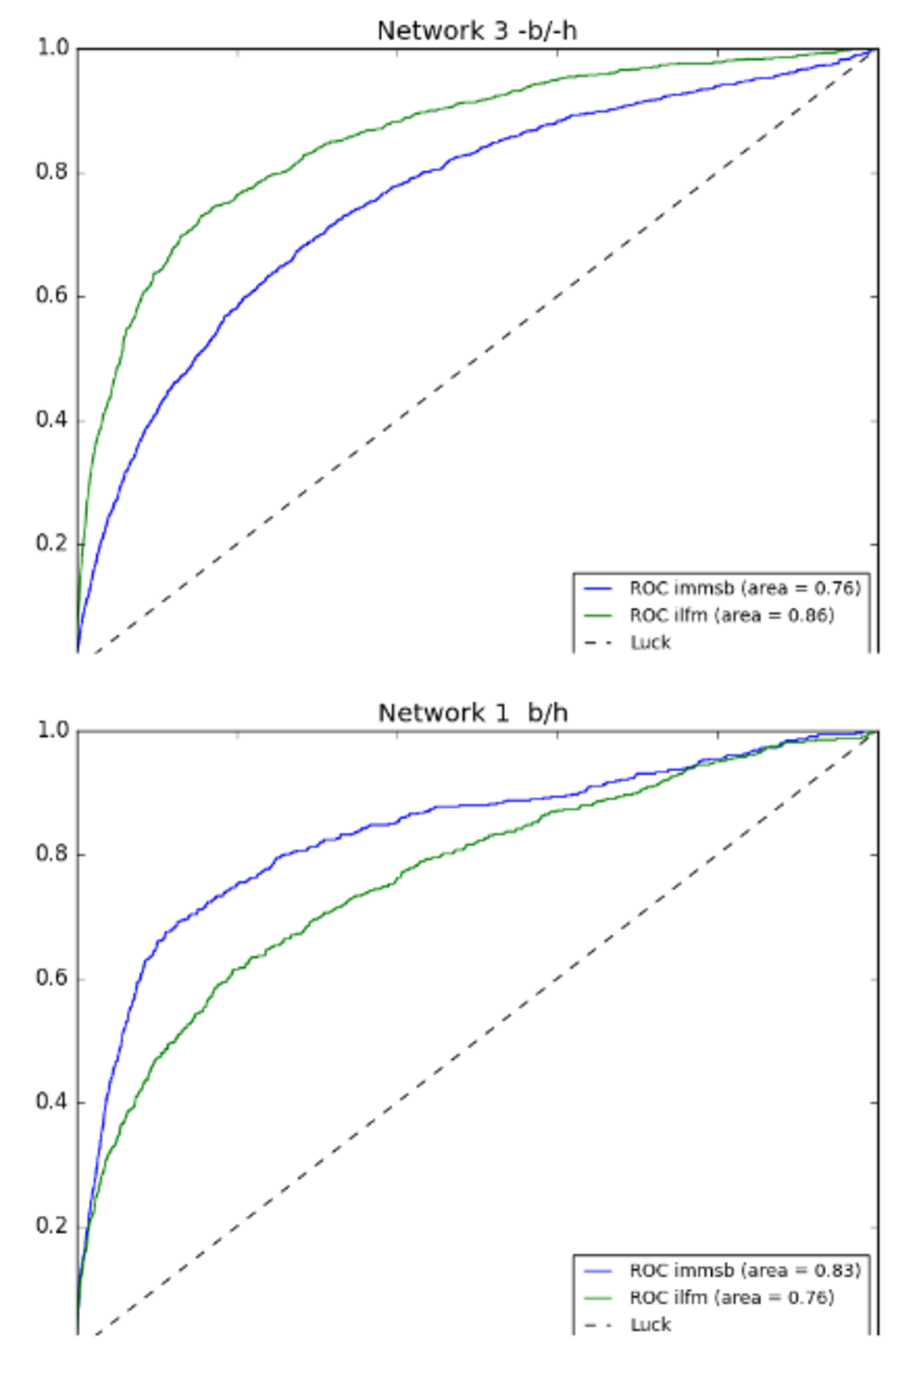
\includegraphics[scale=0.27]{img/auc.pdf}
        \end{figure}
        \end{column}
    \end{columns}

\end{frame}

\begin{frame}[c]{Empirical Results (Preferential attachment II)}
        \begin{figure}[h]
            \caption{Comparison performance of IMMSB and ILFM based on the size of the training set.}
        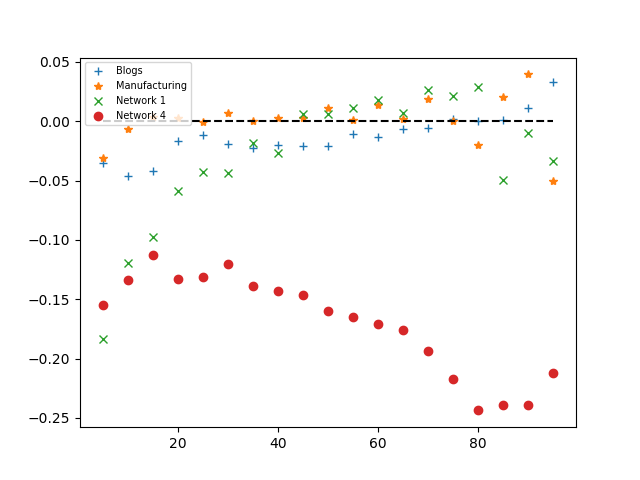
\includegraphics[scale=0.5]{img/testset_max_20_roc_evolution}
        \end{figure}
\end{frame}


\begin{frame}[c]{Empirical Results (Homophily)}
    \begin{figure}[ht]
    \caption{Natural and latent similarities aggregated over all datasets and computed on linked and non-linked pairs of nodes for IMMSB (left) and ILFM (right).}
    \centering
        \begin{subfigure}
             \centering
                 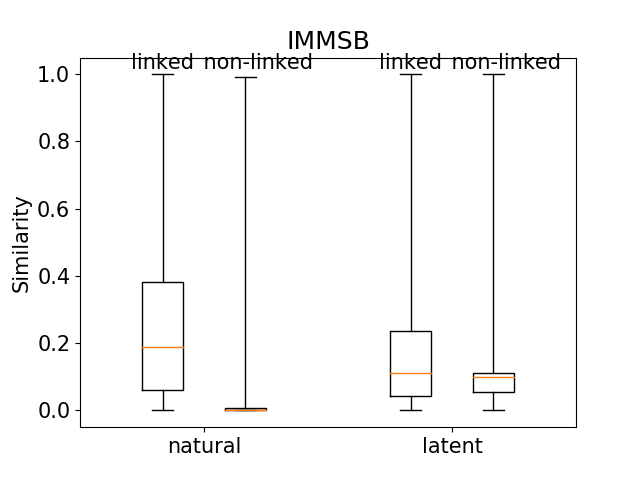
\includegraphics[width=0.4\textwidth]{img/homo_mustach_immsb}
        \end{subfigure}
        \begin{subfigure}
                 \centering
              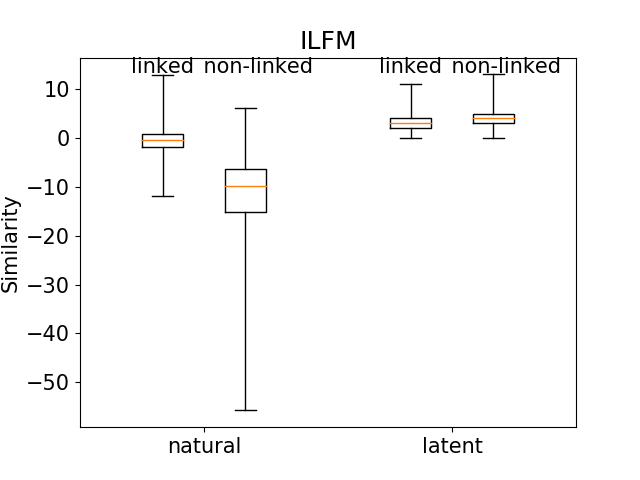
\includegraphics[width=0.4\textwidth]{img/homo_mustach_ilfm}
        \end{subfigure}
        \label{fig:homo_mustach}
    \end{figure}
\end{frame}


\begin{frame}[c]{Conclusion}
    \begin{block}{Wrap up}
    \begin{itemize}
        \item Formal definitions of social networks properties [Homophily and Preferential Attachments].
        \item Study of compliance of IMMSB/ILFM with those properties.
        \item Empirical implication on prediction performances.
    \end{itemize}
    \end{block}


    \begin{block}{Future work}
    \begin{itemize}
        \item Extend to weighted networks (and scalable inference).
        \item Extend to temporal networks. 
        \item Reproducible research/experiments : \hyperlink{http://github.com/dtrckk/pymake}{http://github.com/dtrckd/pymake}

    \end{itemize}
    \end{block}
    

    \pause
    \vspace{1em}
    \textcolor{green}{Thank You}
\end{frame}

%
%
%
%
%
%
%
%
%

\begin{frame}[c]{Limitation and future work}
    Representation Theorem for exchangeable graph \footfullcite{orbanz2015bayesian}.

    \begin{block}{Aldous-Hoover Theorem}
        An array $(Y_{ij})_{{ij}\in \mathbb{N}}$ is jointly exchangeable if and only if :
    \begin{equation}
        Y_{ij} \sim F(U_i, U_j, U_{ij})
    \end{equation}

    \begin{itemize}
        \item With $F: [0,1]^3 \rightarrow [0,1]$ a random measure, 
        \item  $(U_i)_{i\in \mathbb{N}}$ and $(U_{{ij}\in \mathbb{N}})$   i.i.d Uniform[0,1] random variables.
    \end{itemize}
    \end{block}

    A corollary of this theorem is that random exchangeable graph are either \textbf{empty or dense}.
    \vspace{1cm}

    \MVRightarrow{} What network structure and invariance to comply with the Global preferential attachment ?

\end{frame}


\begin{frame}[c]{Characterisation of Burstiness (cont .)}

    Generative Process for IMMSB.

        \begin{figure}[h]
            \caption{IMMSB Simulation.}
        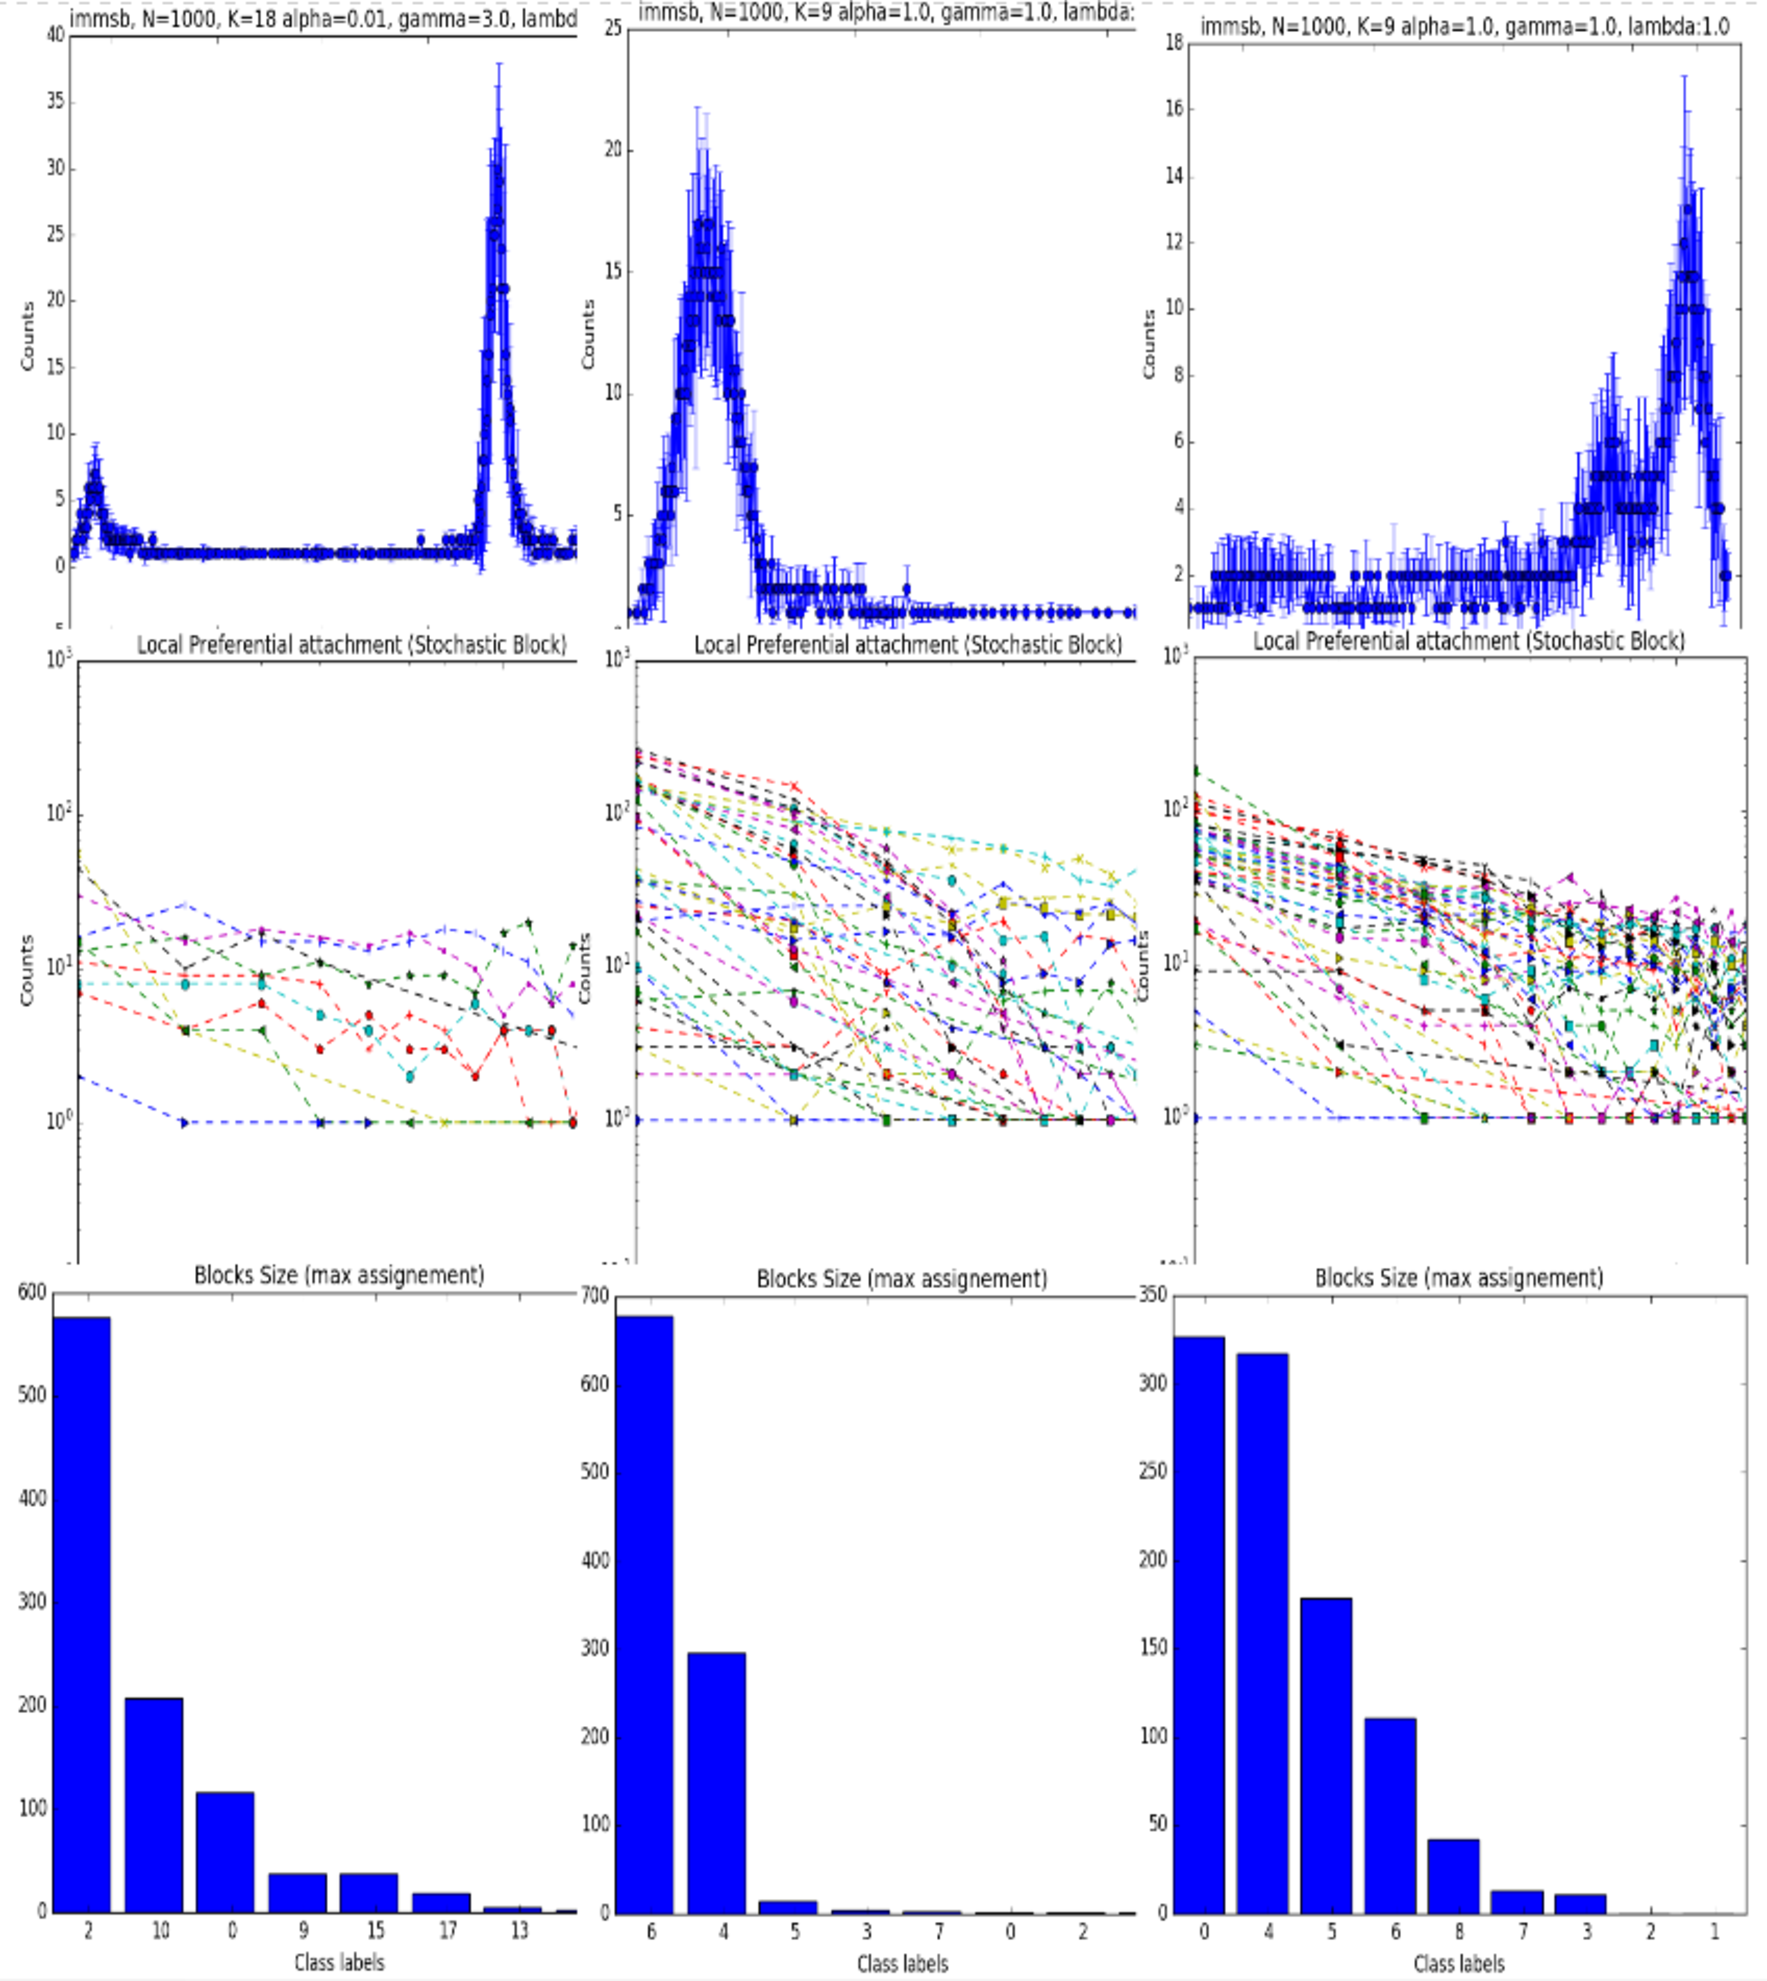
\includegraphics[scale=0.2]{img/mmsb_burst.pdf}
        \end{figure}
\end{frame}

%\begin{frame}[c]{Characterisation of Burstiness (cont .)}
%
%    Generative Process for ILFM.
%
%        \begin{figure}[h]
%        \includegraphics[scale=0.2]{img/ilfm_burst.pdf}
%            \caption{ILFM Simulation.}
%        \end{figure}
%\end{frame}

\begin{frame}[c]{Characterisation of Burstiness (cont .)}

    Is there a proof ?

    \[ P(d_i=n | \alpha) \quad ?\]
    \begin{block}{Problem}
        \begin{itemize}
            \item $d_i$ random variable ?
            \item $P(\bm{Y}_i \mid \alpha, \lambda) = \int_F \int_\Phi p(f_i| \alpha)p(\Phi|\lambda) \prod_{j\neq i} p(f_j|\alpha) p(y_{ij} \mid f_i, f_j, \Phi) \ dF d\Phi$
        \end{itemize}
    \end{block}

    \alert{Intractable}...
\end{frame}


\end{document}


